\section{Processi Organizzativi}
\label{sec:processiorganizzativi}

\subsection{Gestione}

\subsubsection{Scopo}
Questo processo ha come scopo la redazione del documento \emph{Piano di Progetto} e disciplinare la coordinazione del gruppo in merito a:
\begin{itemize}
	\item Ruoli di progetto;
	\item Gestione delle comunicazioni;
	\item Gestione degli incontri;
	\item Sistema di ticketing;
	\item Sistema di versionamento.

\end{itemize}
\subsubsection{Ruoli di progetto}
I ruoli di progetto rappresentano le figure professionali che lavoreranno al progetto.  Ogni membro deve ricoprire ciascun ruolo almeno una volta. Come ciò è pianificato e verificato è specificato nel documento \emph{Piano di Progetto}. I ruoli sono:
\paragraph{Amministratore di Progetto} \Spazio
L'\emph{Amministratore di Progetto} è la figura professionale che si deve occupare di gestire l'ambiente di lavoro del gruppo. Nello specifico deve:
\begin{itemize}
	\item Ricercare nuovi strumenti che migliorino la produttività del gruppo;
	\item Imparare ad utilizzare adeguatamente gli strumenti utilizzati;
	\item Se necessario spiegare agli altri componenti del gruppo come utilizzare correttamente tali strumenti;
	\item Occuparsi del controllo di versione del prodotto;
	\item Occuparsi della configurazione del prodotto.
\end{itemize}
È presente per tutta la durata del progetto.
\paragraph{Analista} \Spazio
L'\emph{Analista} è la figura professionale che si occupa dell'analisi dei requisiti del prodotto e del dominio applicativo. Deve:
\begin{itemize}
	\item Analizzare i requisiti del prodotto. Per fare ciò dovrà parlare in prima persona con il committente;
	\item Analizzare i requisiti di dominio;
	\item Redigere il documento \emph{Studio di Fattibilità};
	\item Redigere il documento \emph{Analisi dei Requisiti}.
\end{itemize}
È presente solamente nella fase iniziale del progetto.
\paragraph{Progettista} \Spazio
Il \emph{Progettista} è la figura professionale che si occupa della progettazione del prodotto. Deve
\begin{itemize}
	\item Comprendere a fondo i requisiti nel documento \emph{Analisi dei Requisiti};
	\item Progettare un'architettura per il prodotto;
	\item Scegliere le tecnologie che si utilizzeranno per realizzare il prodotto, in modo tale che essere permettano di soddisfare i requisiti;
	\item Redigere la documentazione tecnica per il prodotto software;
	\item Redigere il documento \emph{Manuale Sviluppatore}.
\end{itemize}
È presente nella fase di progettazione del prodotto software e \emph{può} seguire il progetto fino al termine.
\paragraph{Verificatore} \Spazio
Il \emph{Verificatore} è la figura professionale che si occupa dell'attività di verifica. Deve
\begin{itemize}
	\item Verificare che ciascuna attività svolta sia conforme alle norme stabilite nel progetto;
	\item Redigere il documento \emph{Piano di Qualifica}.
\end{itemize}
È presente per l'intera durata del progetto.
\paragraph{Programmatore} \Spazio
Il \emph{Programmatore} è la figura professionale che si occupa della codifica del prodotto. Deve
\begin{itemize}
	\item Scrivere il codice  del prodotto software che rispetti le decisioni del \emph{Progettista};
	\item Redigere il documento \emph{Manuale Utente}.
\end{itemize}
È presente durante la fase di codifica del prodotto.
\paragraph{Project Manager} \Spazio
Il \emph{Project Manager} è la figura professionale funge da punto di riferimento per il gruppo, il fornitore e il committente in merito al progetto che amministra. Deve
\begin{itemize}
	\item Organizzare incontri interni ed esterni;
	\item Pianificare le attività svolte dal gruppo, suddividendole in compiti;
	\item Individuare per ciascun compito un membro del gruppo per svolgerlo;
	\item Analizzare, monitorare e gestire i rischi.
\end{itemize}
È presente per l'intera durata del progetto.
\subsubsection{Procedure}
\paragraph{Gestione delle comunicazioni}
\subparagraph{Comunicazioni interne} \Spazio
\label{comInterne}
Le comunicazioni interne sono gestite con la piattaforma \gl{Slack}. Essa rende possibile creare un \gl{workspace} comune al gruppo suddiviso in più \gl{canali di comunicazione}, ad ognuno dei quali sono associati uno scopo ed un sottoinsieme dei membri del gruppo. \emph{Slack} permette anche a due componenti del gruppo di mandarsi messaggi privati. Il maggiore vantaggio rispetto all'utilizzo di un'applicazione di messaggistica come \gl{Telegram} o \gl{Whatsapp} sta nel poter creare uno spazio di comunicazione condiviso che permetta di gestire più categorie di comunicazioni in un singolo \emph{workspace}. % questo riguardalo
\subparagraph{Comunicazioni esterne} \Spazio
La gestione delle comunicazioni esterne è compito del $Project$ $Manager$. Egli deve utilizzare l'indirizzo di posta elettronica:
$$\textbf{sweeftyteam@gmail.com}$$
Il \emph{Project manager} se lo ritiene opportuno può informare i membri del gruppo delle eventuali comunicazioni esterne tramite il canale Slack \emph{\#email}.

\paragraph{Gestione degli incontri}
\subparagraph{Incontri interni} \Spazio
Gli incontri interni del gruppo devono essere organizzati dal \emph{Project Manager}. Egli deve:
\begin{enumerate}
	\item Proporre tramite il canale Slack \emph{incontri} una data, un'ora, un luogo e una motivazione per organizzare l'incontro. La data in cui ciò avviene deve essere almeno a due giorni di distanza dalla data proposta per incontrarsi. Quest'ultima regola può essere ignorata solamente nel caso in cui fosse strettamente necessaria una riunione tempestiva;

	\item Raccogliere tramite il \gl{bot} Slack \gl{Simple Poll} le risposte di partecipazione o assenza dei membri. Esse devono essere date entro e non oltre 24 ore di tempo dall'apertura del sondaggio;

	\item Se almeno cinque membri avranno dato conferma di presenza il \emph{Project Manager} conferma che l'incontro si svoltge con i parametri definiti nel punto 1.
	      Se le conferme di presenza sono tre o quattro starà al \emph{Project Manager} decidere fra:
	      \begin{itemize}
		      \item Confermare l'incontro con solo coloro che hanno confermato al presenza;
		      \item Tornare al punto 1 cambiando i parametri data e/o ora ed eventualmente luogo.
	      \end{itemize}
	      Tale decisione deve prendere in considerazione i benefici che porterebbe organizzare un incontro con tre o quattro membri e gli svantaggi che si avrebbero posticipando l'incontro.
	      Se le conferme sono meno di tre sarà necessario tornare al punto 1 cambiando i parametri data e/o ora ed eventualmente luogo.
\end{enumerate}
Tutti i membri del team possono chiedere di organizzare un incontro al \emph{Project Manager}, specificando una motivazione. Se quest'ultima è ritenuta sufficiente per organizzare un incontro si procede ad avviare la procedura sopra descritta.
\\Inoltre, ad ogni incontro, un membro del gruppo viene scelto dal \emph{Project Manager} per stilare il verbale. Egli deve creare un file contenente un riassunto scritto di ciò di cui si è discusso e ciò che è stato deciso, secondo le modalità riportate in \ref{verbali}.

\begin{figure}
	\centering
	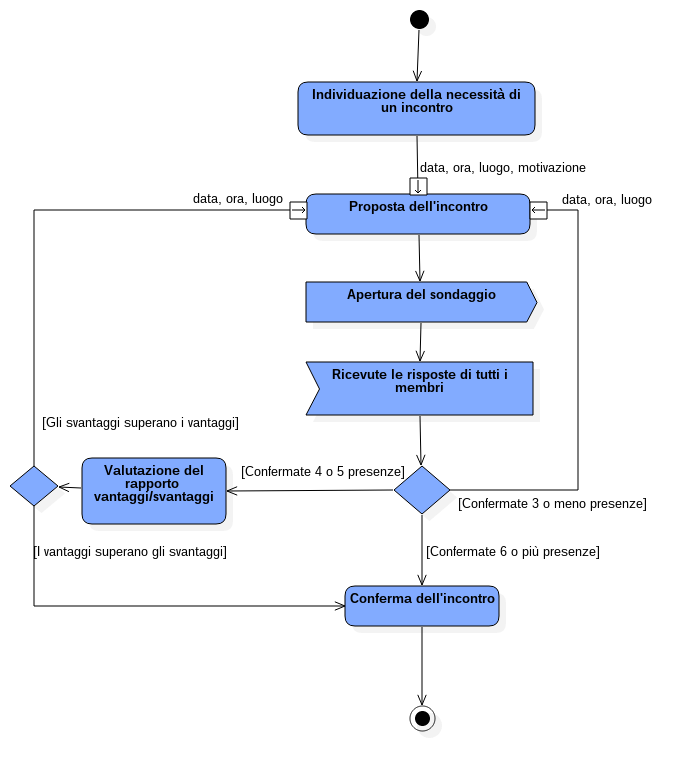
\includegraphics[width=1\textwidth]{Images/umlincontri.png}
	\caption{Diagramma della procedura di organizzazione di un incontro interno}
\end{figure}

\subparagraph{Incontri esterni} \Spazio
Gli incontri esterni devono essere organizzati dal \emph{Project Manager}. È suo compito mettersi in contatto con il committente o il proponente tramite email e determinare data, ora e luogo dell'incontro. Quando ciò è definito deve avvisare i membri del gruppo sul canale Slack \emph{\#incontri}. Anche per gli incontri esterni ciascun membro del gruppo può richiedere che venga organizzato un incontro con il committente o il proponente, specificandone la motivazione. Se essa è giudicata adeguata dal \emph{Project Manager} egli deve procedere ad organizzare tale incontro. È anche suo compito incaricare uno dei presenti di redigere un verbale scritto.
\paragraph{Gestione degli strumenti di coordinamento}
\subparagraph{Ticketing} \Spazio
Per la gestione del sistema di ticketing si utilizza la piattaforma \gl{Wrike}. Essa permette di definire un insieme di tasks. Ad ognuno di essi viene assegnato un nome, una breve descrizione,e un membro che sia incaricato di portarlo a termine, una data di inizio e una data entro la quale il \gl{task} deve essere completato. Il \emph{Project Manager} deve creare i tasks ed assegnare un membro a ciascuno di essi. Una volta raggiunta la data di inizio, l'incaricato di svolgerlo deve portarlo a termine entro e non oltre la data stabilita per la fine. Quando fa ciò deve impostare sulla piattaforma Wrike che tale task è stato completato. Ogni membro del gruppo è tenuto a controllare almeno una volta al giorno la piattaforma per controllare se gli sono stati assegnati nuovi compiti.

\subparagraph{Struttura del worskspace di comunicazioni interne} \Spazio
Come detto in \ref{comInterne} lo strumento utilizzato per le comunicazioni interne è Slack. Il workspace del gruppo è organizzato nei seguenti canali:
\begin{itemize}
	\item \textbf{\#general} è il canale nel quale il gruppo si scambia informazioni per l'appunto di carattere generale, per esempio domande su come utilizzare una \gl{feature} di un determinato strumento piuttosto che avvisare gli altri di essere in anticipo per un incontro;
	\item \textbf{\#incontri} ha lo scopo di organizzare gli incontri interni al gruppo. Qui vengono effettuati i sondaggi di partecipazione tramite il bot \emph{Simple Poll} e successivamente è confermato o meno l'incontro dal \emph{Project Manager};
	\item \textbf{\#todo} ha lo scopo di informare gli altri membri del gruppo che una certa porzione di un determinato task non è completa e potrà essere completata solo dopo che saranno state determinate delle norme nel gruppo. È compito di chi lascia il task incompleto informare gli altri tramite questo canale. I messaggi devono seguire la forma:
	      $$[TODO]\text{ spiegazione del problema}$$
	\item \textbf{\#email} è il canale nel quale il \emph{Project Manager} inserisce le risposte che vengono fornite da entità esterne alla casella mail del gruppo, se lo ritiene necessario o utile.
\end{itemize}

\paragraph{Gestione degli strumenti di versionamento}
\subparagraph{Repository} \Spazio
La piattaforma di \gl{hosting} scelta per il repository è GitHub. Si utilizza una licenza "educational", che permette di avere fino a cinque repository private condivise. Di queste solamente una è effettivamente utilizzata. È organizzata come descritto in \ref{repoStruct}
\subparagraph{Struttura del repository}\Spazio
\label{repoStruct}
La struttura è la seguente\\
\begin{center}
	\begin{forest}
		for tree={
		font=\ttfamily,
		grow'=0,
		child anchor=west,
		parent anchor=south,
		anchor=west,
		calign=first,
		edge path={
				\noexpand\path [draw, \forestoption{edge}]
				(!u.south west) +(7.5pt,0) |- node[fill,inner sep=1.25pt] {} (.child anchor)\forestoption{edge label};
			},
		before typesetting nodes={
				if n=1
					{insert before={[,phantom]}}
					{}
			},
		fit=band,
		before computing xy={l=15pt},
		}
		[SWEefty
			[Docs
					[CommonImages]
					[Template]
					[RR]
					[RP]
					[RQ]
					[RA]
			]
			[Code]
		]
	\end{forest}
\end{center}
dove:
\begin{itemize}
	\item \texttt{SWEefty} rappresenta la radice dello spazio di lavoro;
	\item \texttt{Docs} è la directory in cui sono inseriti tutti i documenti formali;
	\item \texttt{Code} è la directory dove è inserito il codice;
	\item \texttt{CommonImages} contiene le immagini comuni a tutti i documenti, per esempio il logo del gruppo;
	\item \texttt{Template} contiene i files che compongono la struttura comune a tutti i documenti che verranno redatti;
	\item \texttt{RR} contiene tutti i documenti da consegnare per la Revisione dei Requisiti;
	\item \texttt{RP} contiene tutti i documenti da consegnare per la Revisione di Progettazione;
	\item \texttt{RQ} contiene tutti i documenti da consegnare per la Revisione di Qualifica;
	\item \texttt{RA} contiene tutti i documenti da consegnare per la Revisione di Accettazione;
\end{itemize}

\subparagraph{Norme sui nomi dei files} \Spazio
Ciascun file deve essere denominato seguendo la codifica:

\begin{center}
	\texttt{NomeDelFile[\char`_vX.Y.Z].ext}
\end{center}
Dove NomeDelFile rappresenta il nome del file e ciascuna parola che compone tale nome è identificata da una lettera maiuscola. Ext rappresenta l'estesione del file. La parte all'interno delle parentesi quadre è quella che indica la versione in cui il file si trova e X,Y e Z rappresentano la specifica versione. È opzionale in quanto non tutti i documenti hanno un controllo di versione, per esempio i verbali. Nel caso in cui dovessero essere presenti lettere accentate nel nome, l'accento deve essere ignorato e inserita semplicemente la lettera non accetata. Per esempio il file sorgente .tex del documento \emph{Studio di Fattibilità v1.0.0} è denominato \texttt{StudioDiFattibilita\_v1.0.0.tex}.

\subparagraph{Estensioni ammesse} \Spazio
I file che si trovano effettivamente nella directory \texttt{Docs} sono solamente immagini .jpg e .png, file sorgente \LaTeX $\text{ }$ .tex . Tutti i file.pdf compilati e i prodotti intermedi del programma per la compilazione di file .tex \texttt{pdflatex} .aux, .dvi, .fls, .log, .out, .toc verranno inseriti nel file \texttt{.gitignore} che rende la loro presenza trasparente a \gl{Git}.

\subparagraph{Norme di branching e merging} \Spazio
Git mette a disposizione il comando \texttt{branch} per poter creare un nuovo ramo di lavoro all'interno della repository, indipendente da quello principale. I rami possono essere a loro volta divisi in sottorami figli, così come uniti ad altri tramite il comando \texttt{merge}. Si deve creare un nuovo branch nei seguenti casi:
\begin{itemize}
	\item Viene istanziato un nuovo documento che non sia un verbale;
	\item Più componenti del gruppo stanno lavorando al medesimo documento ed è necessario inserire un nuovo file che abbia estensione .tex;
	\item Deve essere implementata nel codice un'unità.
\end{itemize}
Tutte le modifiche ai documenti e al codice devono essere eseguite all'interno del nuovo branch. Una volta completate sarà possibile eseguire il merging del branch figlio con il padre. Questa operazione deve essere eseguita dall'\emph{Amministratore di Sistema} che dovrà correggere eventuali conflitti.

\subparagraph{Norme su commit}\Spazio
Ogni volta che viene effettuata una modifica significativa ad un file oppure una serie di modifiche strettamente correlate su più files, va utilizzato il comando \texttt{commit} di git. In esso ci deve specificare un messaggio che descriva brevemente ciò che è stato fatto. I caratteri di questo messaggio non devono essere più di 80. Deve seguire la semantica
$$\text{[sigla file] breve descrizione}$$
Per esempio l'aggiunta della sezione "XYZ" al file \texttt{NormeDiProgetto\_v1.0.0.tex} comporterebbe scrivere come messaggio informativo "[NDP] Aggiunta sezione XYZ". Prima di eseguire una \texttt{commit} va aggiornato il Diario delle Modifiche come descritto in \ref{registroModifiche}

\paragraph{Gestione dei rischi} \Spazio
La gestione dei rischi è compito del \emph{Project Manager}. Egli li deve identificare, inserirli nel $Piano\text{ }di\text{ }Progetto$ e valutare una strategia per affrontarli. Nel caso in cui si presentassero nuovi rischi non osservati sarà sempre compito del \emph{Project Manager} inserirli nel \emph{Piano di Progetto}. Durante tutta la durata del progetto deve inoltre monitorare tali rischi e, solo se necessario, ridefinire le strategie di progetto.

\subsubsection{Strumenti}

\paragraph{Sistema Operativo} \Spazio
I sistemi operativi utilizzati dai membri del gruppo sono:
\begin{itemize}
	\item Ubuntu GNOME 17.10 x64;
	\item Ubuntu 17.10 x64;
	\item Windows 10 Home x64;
	\item MacOS High Sierra x64;
\end{itemize}

\paragraph{Slack}\Spazio
Slack è lo strumento adottato per gestire le comunicazioni interne al gruppo. Esso è gratuito e permette di creare in un workspace comune con più canali di comunicazione, contrassegnati da un cancelletto. Permette anche l'integrazione con altri strumenti utilizzati, quali \gl{Dropbox}, Wrike e GitHub. Queste \gl{major features} lo rendono preferibile ad altre applicazioni di messaggistica quali Telegram o Whatsapp, più idonee ad un uso personale.

\paragraph{Wrike} \Spazio
Wrike è lo strumento adottato per gestire il sistema di ticketing. È una piattaforma online che mette a disposizione anche una applicazione per dispositivi mobili per la gestione di tasks all'interno di un progetto. Il principale motivo per il quale risulta comodo da utilizzare è che il sistema, una volta definiti un insieme di compiti e ad essi sono stati  assegnate date di inizio e di fine, permette di avere più viste degli stessi: una lista testuale, una tabella, uno stream, una board o un \gl{diagramma di Gantt}. \\ Wrike è uno strumento a pagamento. La licenza utilizzata dal gruppo è quella per studenti ed ha una durata di 750 giorni.

\paragraph{Github} \Spazio
Github è la piattaforma scelta per l'hosting della repository. Essa si basa sul sistema di versionamento git, descritto in \ref{descGit}. Ha piani di sottoscrizioni gratuiti o a pagamento. La differenza sta nella possibilità di disporre di repository private. Con l'edizione "educational" da noi utilizzata si possono ottenere gratuitamente fino a cinque repository gratuite. GitHub offre inoltre un gran numero di tools utili per lo sviluppo aggiuntivi, come la gestione tramite interfaccia web delle \gl{issues}.

\paragraph{Git} \Spazio
Git\label{descGit} è il sistema per il controllo del versionamento utilizzato. Ha un'architettura distribuita ed è l'unico sistema di controllo di versione supportato da GitHub. Rispetto ad altri strumenti di controllo di versionamento, come \gl{Mercurial}, ha un numero molto maggiore di comandi, il che rende difficile per un neofita l'utilizzo da riga di comando di git.

\paragraph{Gitkraken} \Spazio
\gl{Gitkraken} è un'applicazione desktop \gl{multipiattaforma} che semplifica l'utilizzo di git, esponendo una chiara interfaccia grafica che si sostituisce all'utilizzo di git da riga di comando. Grazie a ciò rende più semplice imparare ad usare lo strumento di versionamento e dà una visualizzazione grafica dello storico della repository.

\begin{figure}[H]
	\centering
	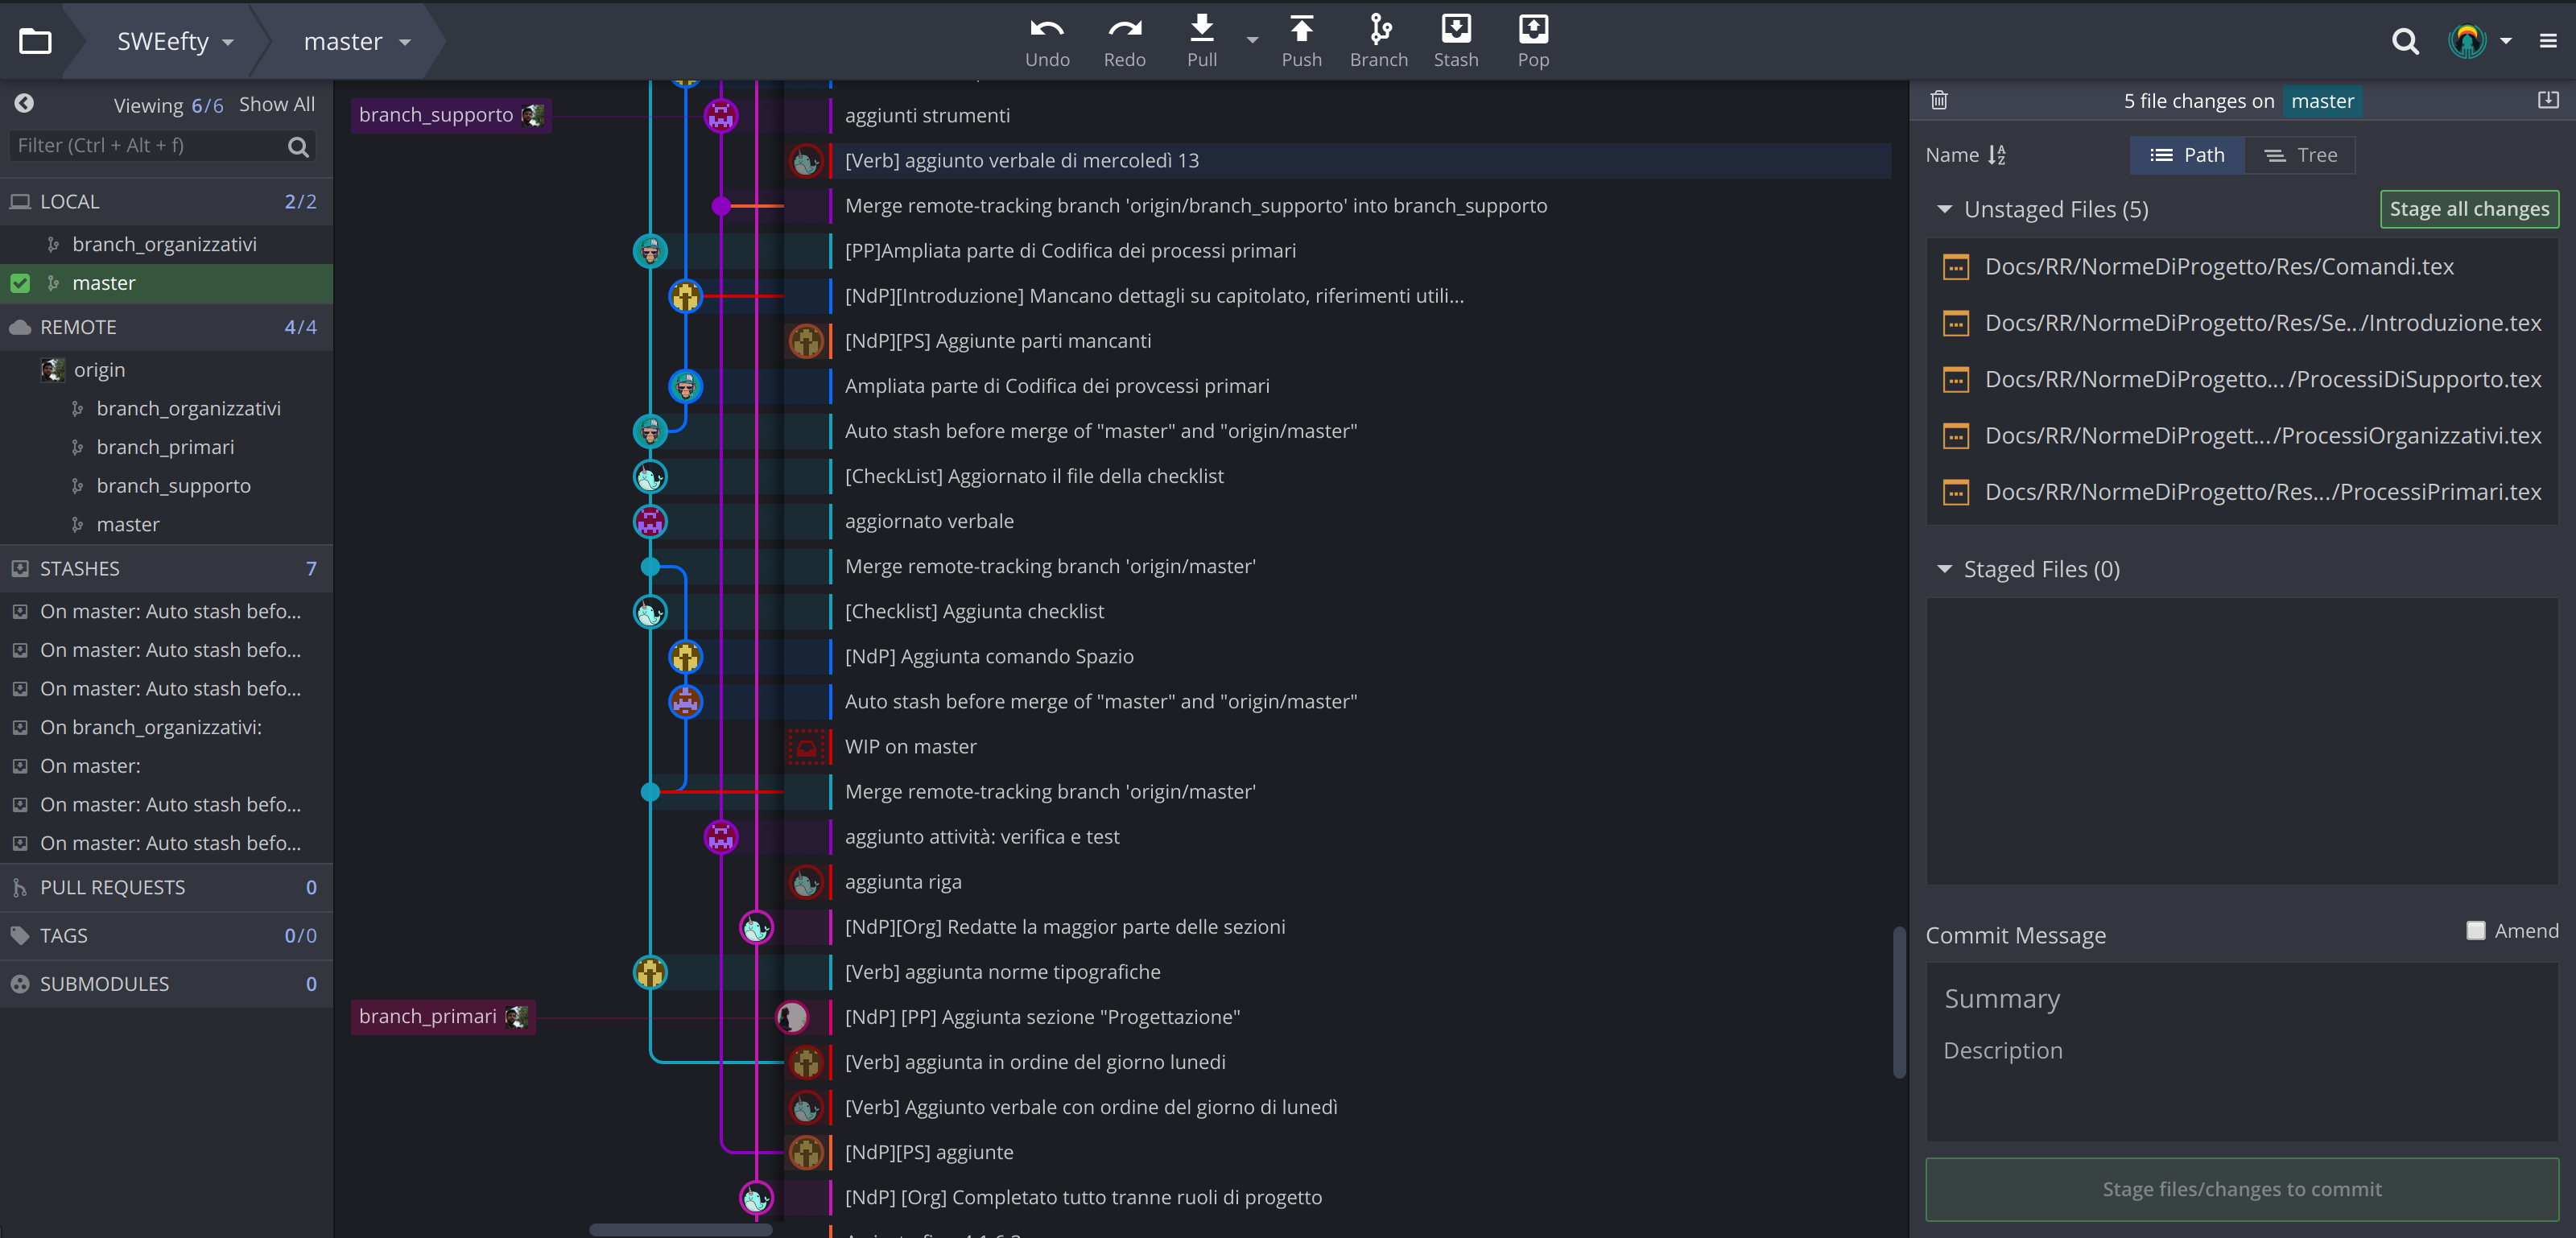
\includegraphics[width=1\textwidth]{Images/gitkraken.png}
	\caption{Interfaccia grafica del software Gitkraken su Ubuntu GNOME}
\end{figure}

\subsection{Formazione}
\label{sec:formazione}

\subsubsection{Scopo}
Lo scopo del processo di formazione è quello di formare i membri del gruppo riguardo alle tecnologie che si andranno ad utilizzare nell'implementazione del prodotto. Il successo del progetto dipende in larga parte dalla preparazione dei componenti del gruppo, dunque è opportuno che essi vengano istruiti a dovere ed eventualmente aggiornino le loro conoscenze ereditate da esperienze passate.
\subsubsection{Attività}
	\paragraph{Studio delle tecnologie richieste} \Spazio
	Per poter formare adeguatamente i membri del gruppo è necessario conoscere le tecnologie che essi andranno ad utilizzare. Esse appartengono a due categorie: 
	\begin{enumerate}
		\item \textbf{Richieste}: la loro adozione viene richiesta esplicitamente dal committente, non esiste un margine di scelta;
		
		\item \textbf{Scelte}: la loro adozione viene fatta in base alla scelta del \emph{Progettista}, che deve eseguire una attenta analisi del panorama tecnologico disponibile sul mercato. Deve valutare il rapporto costi-benefici di ciascuna tecnologia, tenendo conto anche della difficoltà che si avranno nella formazione del personale.
	\end{enumerate}
	L'identificazione delle tecnologie deve essere fatta il prima possibile per permettere di formare rapidamente il personale e dunque eseguire la progettazione e l'implementazione del prodotto nei tempi prestabiliti. Per questo motivo deve essere la prima attività eseguita dopo l'analisi. 

	\paragraph{Sviluppo di materiale di formazione} \Spazio
	Una volta identificate le tecnologie l'\emph{Amministratore} deve predisporre il materiale necessario all'apprendimento. Il materiale può essere sviluppato: 
	\begin{itemize}
		\item \textbf{Internamente}: se prodotto internamente al gruppo dall'\emph{Amministratore};
		\item \textbf{Esternamente}: se prodotto da entità esterne al gruppo, come siti web o sviluppatori.
	\end{itemize}
	Tutto il materiale di formazione deve essere inserito nella cartella Dropbox del gruppo, in una sottocartella denominata \emph{Tutorials}. Essa è organizzata per argomento: ciascuna tecnologia per la quale si possiede del materiale dovrà avere una relativa cartella denominata con il nome della tecnologia stessa. Per esempio tutto il materiale relativo a \LaTeX\text{ } dovrà essere riposto nella cartella \texttt{Tutorials/LaTeX}. Il materiale presente in rete deve essere inserito nella cartella riferendosi all'\gl{URL} che lo rappresenta. Ogni cartella contentente il materiale riguardante una tecnologia deve contenere un file chiamato \texttt{links.txt} che contenga tutti gli URL delle risorse in rete. 

	\paragraph{Implementazione del piano di formazione} \Spazio
	Il processo di formazione è individuale. Il \emph{Project Manager} deve assegnare un intervallo di tempo nel quale tutti i membri del gruppo si dovranno formare consultando tutto il materiale presente nella cartella di Dropbox preparata dall'\emph{Amministratore}. Quando questo periodo ha inizio il \emph{Project Manager} deve assegnare a \emph{tutti} i membri del gruppo un \emph{task} su Wrike dove è necessario indichi con precisione il materiale da consultare. Per permettere il tracciamento della formazione ciascun membro del gruppo è tenuto a segnare su Wrike come "completato" il \emph{task} una volta terminata la formazione individuale.


\subsection{Manutenzione dei processi}
\label{sec:manutenzioneProcessi}
\subsubsection{Scopo}
Lo scopo di questo processo è il miglioramento incrementale dei processi istanziati. Tramite tecniche di controllo, misurazione e valutazione dei processi si realizza un ciclo di miglioramento continuo.

\subsubsection{Attività}
	\paragraph{Valutazione di processo} \Spazio
	Ciascun processo deve essere \emph{misurato}. Le modalità di misurazione sono descritte approfonditamente nel documento \emph{Piano di Qualifica v2.0.0}. 
	Una volta eseguite le misurazioni esse dovranno essere mostrate tramite un cruscotto informativo al controllo. Un insieme di misurazioni costituiscono i dati necessari per dare una \emph{valutazione}. Le valutazioni dovranno essere date dal \emph{Project Manager} e costituiranno l'input per \ref{sec:miglioramentoProcesso}. Le modalità di valutazione sono descritte approfonditamente nel documento \emph{Piano di Progetto v2.0.0}. Misurazioni e valutazioni vanno eseguite seguendo le modalità descritte nei relativi documenti.

	\paragraph{Miglioramento di processo} \Spazio
	\label{sec:miglioramentoProcesso}
	Il \emph{Project Manager} deve analizzare le valutazioni relative a ciascun processo. Se esse non sono soddisfacenti, in base ai range descritti nel documento \emph{Piano di Progetto v2.0.0}, allora deve eseguire l'attività di miglioramento di processo. Deve dunque istanziare dei nuovi vincoli relativi al processo, comunicandoli al gruppo tramite un avviso nel canale \emph{\#general} di \emph{Slack}. È compito dell'\emph{Amministratore di Sistema} una volta visionati i nuovi vincoli aggiornare di conseguenza il documento \emph{Norme di Progetto} e tutta la possibile documentazione annessa ai processi coinvolti. 
